\documentclass[border=6pt]{standalone}
\usepackage{amsmath}
\usepackage{tikz}
\usetikzlibrary{arrows.meta}
\begin{document}
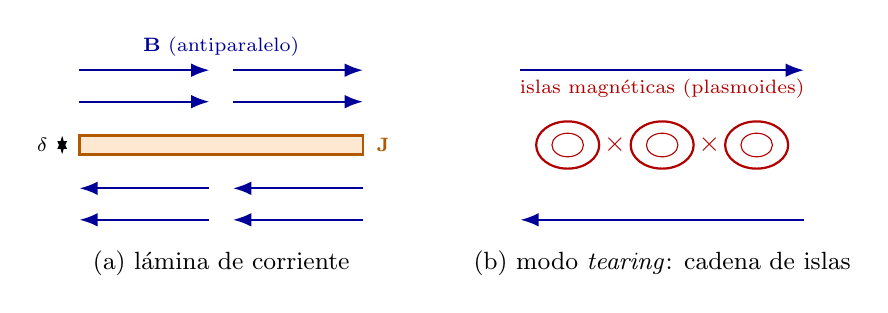
\begin{tikzpicture}[>=Latex,scale=1.0]

% ===== Panel (a): lamina de corriente laminar =====
\begin{scope}
 \node[font=\small] at (2.1,-1.5){(a) l\'amina de corriente};
 \foreach \y in {0.55,0.95}{
   \draw[->,blue!60!black,thick](0.3,\y)--(1.95,\y);
   \draw[->,blue!60!black,thick](2.25,\y)--(3.9,\y);}
 \foreach \y in {-0.55,-0.95}{
   \draw[<-,blue!60!black,thick](0.3,\y)--(1.95,\y);
   \draw[<-,blue!60!black,thick](2.25,\y)--(3.9,\y);}
 \fill[orange!18](0.3,-0.12) rectangle (3.9,0.12);
 \draw[orange!70!black,thick](0.3,-0.12) rectangle (3.9,0.12);
 \node[orange!70!black,font=\scriptsize,right] at (3.95,0){$\mathbf J$};
 \node[blue!60!black,font=\scriptsize] at (2.1,1.25){$\mathbf B$ (antiparalelo)};
 \draw[<->](0.08,-0.12)--(0.08,0.12);
 \node[font=\scriptsize,left] at (0.02,0){$\delta$};
\end{scope}

% ===== Panel (b): tearing -> islas (plasmoides) =====
\begin{scope}[xshift=5.6cm]
 \node[font=\small] at (2.1,-1.5){(b) modo \emph{tearing}: cadena de islas};
 \draw[->,blue!60!black,thick](0.3,0.95)--(3.9,0.95);
 \draw[<-,blue!60!black,thick](0.3,-0.95)--(3.9,-0.95);
 % islas magneticas (O-points)
 \foreach \cx in {0.9,2.1,3.3}{
   \draw[red!70!black,thick] (\cx,0) ellipse (0.40 and 0.30);
   \draw[red!70!black,thin]  (\cx,0) ellipse (0.20 and 0.15);
 }
 % X-points entre islas
 \foreach \cx in {1.5,2.7}{\node[red!70!black] at (\cx,0){$\times$};}
 \node[red!70!black,font=\scriptsize] at (2.1,0.72){islas magn\'eticas (plasmoides)};
\end{scope}

\end{tikzpicture}
\end{document}
